\section{Clustering with RapidMiner}

RapidMiner has different Modules for Clustering already implemented. We apply the k-Means algorithm with mixed measure (euclidean).

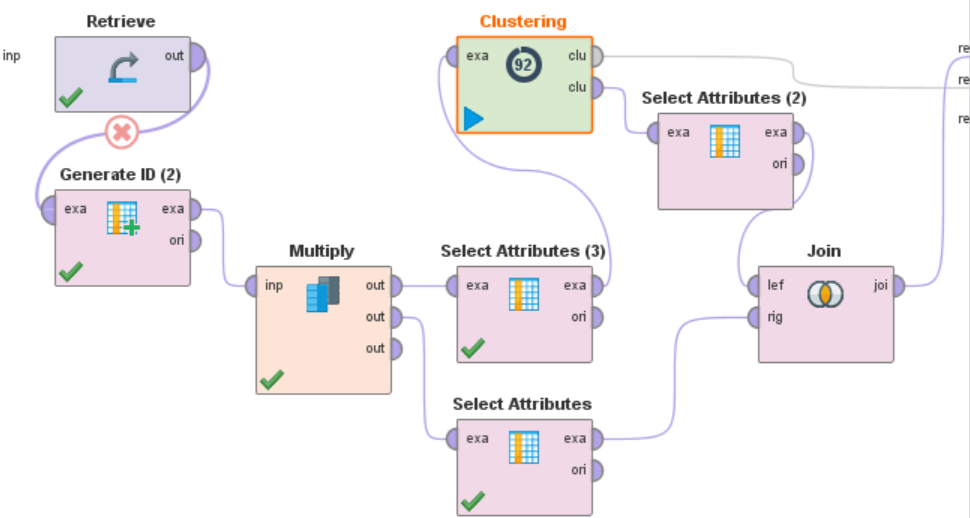
\includegraphics[width=0.9\textwidth]{ClusteringRapid.PNG}


The Process does the following steps:
\begin{description}
	\item[Retrieve] This Block gives the data in the process. For the comparison at the end we also retrieve the original data.
	\item[Nominal to Numerical] This changes the nominal data to numerical data, so that we can apply PCA in the next step
	\item[PCA] Here we apply the PCA reduction to the data with a variance threshold $0.95$
	\item[Clustering] Here the number of Clusters has to be fixed. We decided, that 10 runs should be enough. We can choose between differen measure types and tried mixed euclidean and squared euclidean distance
	\item[Select Attribute] Here we just pick the Strata data for comparing with the clustering
	\item[Join] For comparing the Clustering and the Strata we join the two filtered data sets at the ID
\end{description}

\subsection{Original Data}

Applying this process to the original data you can see without alignment of strata and cluster, that the distribution of cluster and strata is not close to the same.

\ref{fig:OrgDist}. 
\begin{figure}
\centering
\begin{subfigure}{.5\textwidth}
  \centering
  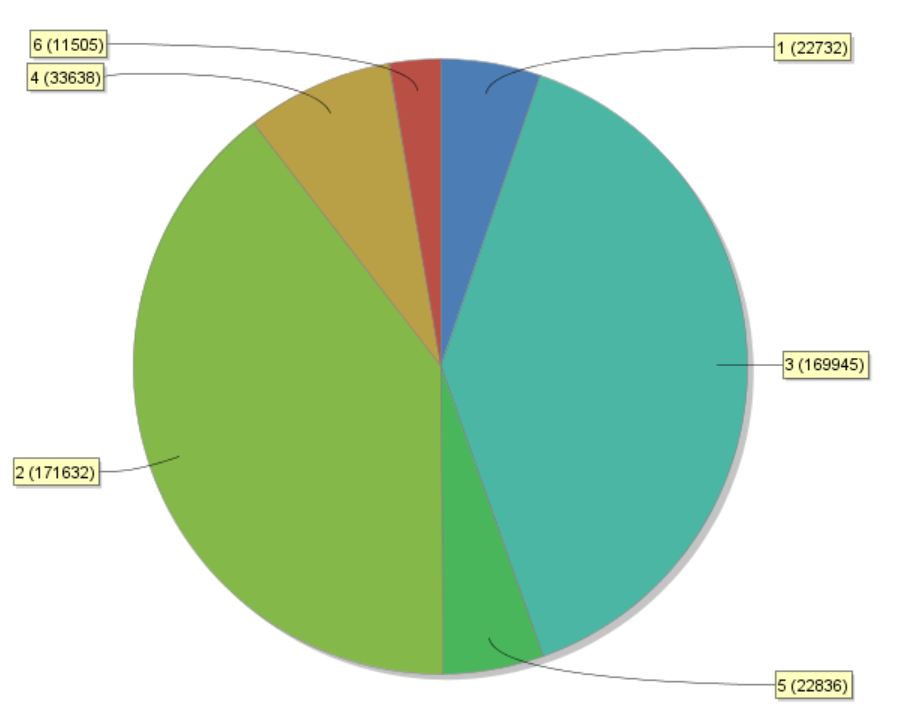
\includegraphics[width=.4\linewidth]{ClusterPCAOrigRapidStrata.PNG}
  \caption{Strata}
  \label{fig:OrgSt}
\end{subfigure}%
\begin{subfigure}{.5\textwidth}
  \centering
  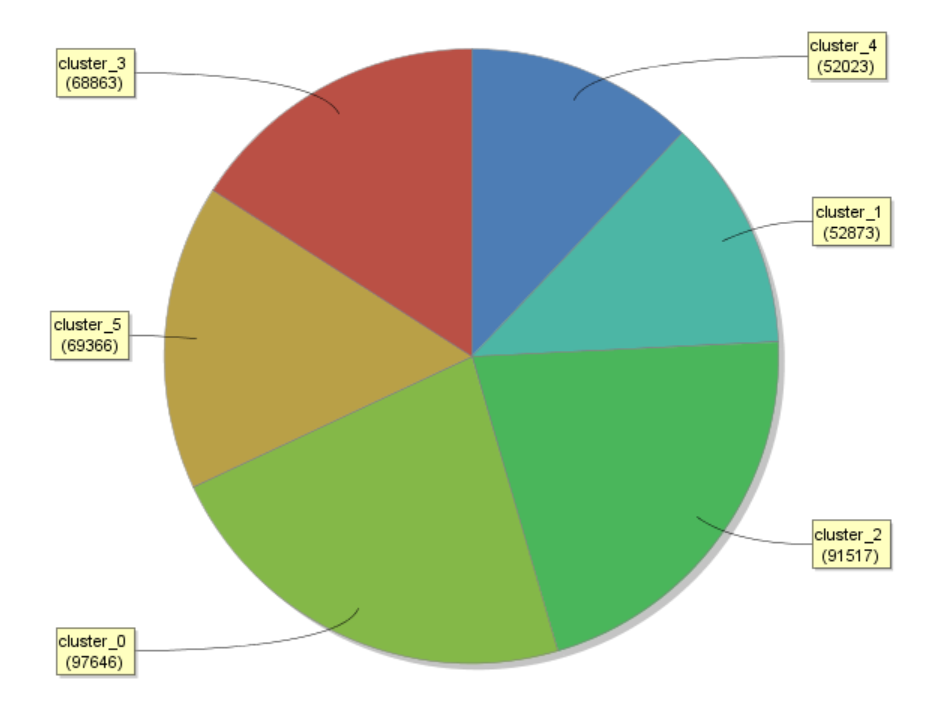
\includegraphics[width=.4\linewidth]{ClusterPCAOrigRapidCluster.PNG}
  \caption{Cluster}
  \label{fig:OrgCl}
\end{subfigure}
\caption{Distribution of original data}
\label{fig:OrgDist}
\end{figure}
